\newpage
\begin{center}
  \textbf{\large 2. Методология}
\end{center}
\refstepcounter{chapter}
\addcontentsline{toc}{chapter}{2. Методология}
\label{method}

\section{Описание метода}
В данном разделе приводится выбор и описание параметров среды для рандомизации, а также методология оценки робастности моделей, где под робастностью понимается способность модели сохранять эффективность в рандомизированных средах.

    \subsection{Выбор параметров среды для варьирования}

        Как и в случае доменной рандомизации, задачей является получить достаточно разнообразное распределение вариаций сцен, такое что потенциальная сцена реального мира лежит в рамках этого распределения. Такой подход подразумевает вариацию множества параметров, как физических, так и визуальных. Далее представлено описание 8 выбранных параметров:

        \begin{enumerate}
            \item Параметры объекта манипулирования (ОМ). Объект манипулирования представляет собой целевой объект, с которым робот непосредственное взаимодействует или манипулирует. Вариации ОМ включают: \textbf{цвет ОМ}, \textbf{текстуру ОМ};

            \item Параметры заднего плана. К заднему плану относятся объекты, являющиеся фоновыми на изображениях, доступных агенту, к таким можно отнести стены, стол, источник освещения. Вариации заднего плана включают: \textbf{цвет заднего плана}, \textbf{текстура заднего плана}, \textbf{цвет источника освещения}, \textbf{отвлекающий объект}. Отличие цвета от текстуры заключается в том, что цвет -- это однородный оттенок, а текстура — детальное изображение на поверхности объекта;

            \item Параметры камеры. Вариации камеры включают: \textbf{смещение камеры};

            \item Физические параметры объектов. Вариации физических параметров включают: \textbf{масса объектов}, \textbf{коэффициенты трения объектов}.
        \end{enumerate}

        Выбранные вариации соответствуют потенциальным отличиям между исходным доменном и целевым, а также возмущениям, присущим среде реального мира. 

    \subsection{Процедура варьирования параметров}
         \label{method_randomization}
        Метод варьирования параметров был заимствован также из доменной рандомизации \cite{Peng_2018}. В зависимости от природы параметра было выбрано 3 метода варьирования:

        \begin{enumerate}
            \item \textbf{Непрерывный скалярный случай.} Если параметр принимает некоторое скалярное значение $a \in \mathbb{R}$, то его распределение может быть выбрано, как:
            \begin{equation}
                x \sim Uniform(x^* - \varepsilon, x^* + \varepsilon),
            \end{equation}
            где $x^*$ -- значение параметра для исходной, не рандомизированной среды; $\varepsilon$ --  настраиваемый параметр; $Uniform$ -- равномерное распределение. К параметрам этого типа можно отнести коэффициенты трения, массу. 

            \item \textbf{Непрерывный многомерный случай.} Если параметр принимает не скалярное значение, а некоторый вектор размера $n$: $x \in \mathbb{R}^n$, то распределение этого вектора может быть выбрано, как: 

                \begin{equation}
                    x_i \sim \mathrm{Uniform}(x_i^* - \varepsilon_i, x_i^* + \varepsilon_i), \quad \forall i \in {1, \dots, n},
                \end{equation}

            где $x_i^*$ -- значение элемента вектора для исходной, не рандомизированной среды; $\varepsilon_i$ --  настраиваемый параметр. К параметрам этого типа можно отнести цвета объектов.
 
            \item \textbf{Дискретный случай.} Некоторые параметры не могут быть представлены в непрерывном пространстве. Пусть параметр принимает некоторое значение $x \in \mathcal{X}$, где $\mathcal{X}$ - ограниченное множество допустимых вариаций, тогда распределение для такого параметра может быть представлено в виде:
            
            \begin{equation}
                x \sim \mathrm{Uniform}(\mathcal{X}).
            \end{equation}

            К этому типу параметром, например, относятся текстуры, тогда в качестве $x$ выступает конкретная текстура, то есть изображение, равновероятно выбранная из заданного множества текстур $\mathcal{X}$.
             
        \end{enumerate}

            Полный список возможных рандомизаций, их тип и описание приведен в таблице \ref{tab:randomization}.
            \begin{table}[ht]
                \caption{Список вариаций предлагаемого метода}
                \label{tab:randomization}
                \centering{
                  \begin{tabular}{|p{3.5cm}|p{3cm}|p{8cm}| }
                    \hline
                    \mbox{Рандомизация} & Тип & Описание \\ \hline 
                    \mbox{Исходная} среда & - & Среда, в которой проходило обучение, или приближенная к ней \\ \hline
                   \multicolumn{3}{|c|}{\textit{Визуальные параметры}} \\ \hline  
                   \mbox{Текстура} ОМ & \multirow{2}{3cm}[-0.4cm]{Дискретный} & \multirow{2}{8cm}{Рандомизация изображения для текстуры объекта, выбирается из заданного набора} \\ \cline{1-1}
                   \mbox{Текстура} \mbox{заднего} \mbox{плана} & & \\ \hline
                   \mbox{Цвет} ОМ & \multirow{3}{3cm}[-0.8cm]{Непрерывный, $\mathbb{R}^3$} & \multirow{3}{8cm}{Рандомизация цвета объекта, путем выбора из заданного промежутка значения насыщенности для каждого канала RGB} \\ \cline{1-1}
                   \mbox{Цвет} \mbox{заднего} \mbox{плана} &  & \\ \cline{1-1}
                   \mbox{Цвет} \mbox{источника} \mbox{освещения} & & \\ \hline
                   \mbox{Отвлекающий} \mbox{объект} & Непрерывный, $\mathbb{R}^6$ & Рандомизация положения отвлекающего объекта, генерируется координата объекта $x \in \mathbb{R}^3$ и ориентация в углах Эйлера $\Delta \theta \in \mathbb{R}^3$. Отвлекающий объект его внешний вид и другие характеристики определяется исходя из задачи \\ \hline
                   \mbox{Смещение} \mbox{камеры} & Непрерывный, $\mathbb{R}^6$ & Рандомизация положения камеры, генерируется линейное смещение $\Delta x \in \mathbb{R}^3$ и смещения по ориентации в углах Эйлера $\Delta \theta \in \mathbb{R}^3$  \\ \hline
                    \multicolumn{3}{|c|}{\textit{Физические параметры}} \\ \hline  
                     Масса \mbox{объектов} & \multirow{1}{3cm}[-0.4cm]{Непрерывный, $\mathbb{R}$} & Рандомизация значения массы объектов, выбирается из заданного промежутка \\ \hline
                     Трения \mbox{объектов} & \multirow{1}{3cm}[-0.6cm]{Непрерывный, $\mathbb{R}^2$} & Рандомизация коэффициентов трения покоя $k_0$ и трения скольжения $\mu$ объектов, путем выбора из заданного промежутка \\ \hline
                  \end{tabular}
                }
            \end{table}
            
            Настраиваемые параметры, такие как $\varepsilon$ для непрерывных случаев или элементы множества $\mathcal{X}$ для дискретного случая, зависят от задачи, отличий между исходным и целевым доменами, а также от природы возможных возмущений целевого домена. 
       
        \subsubsection{Отсутствие явной исходной среды}
            
            При исследовании обученной модели, возможна ситуация, когда исходная среда недоступна или неизвестна, например, если модель была обучена не реальных данных. В таком случае неизвестны и исходные параметры $x^*$ для определения параметров распределения. Для решения этой проблемы предлагается два метода:

            \begin{itemize}
                \item Некоторым образом идентифицировать параметры реального мира, то есть получить оценку интересующего параметра $\hat{x}^*$, например аналогично методам из работы Simpler;
                \item Зафиксировать приблизительное значение параметра $\hat{x}^*$ и выбрать достаточно большое значение для $\varepsilon$, чтобы распределение вариаций с большей вероятностью покрывало целевой домен.
            \end{itemize}

            Выбор конкретного метода зависит от задачи и доступных ресурсов. Первый метод может оказать дорогостоящим, но может дать более точные результаты. Второй метод более доступный, но полученные результаты могут оказаться недостаточно релевантными, в случае, если итоговое распределение сцен радикально отличается от тех, что использовались при обучении. 

    \subsection{Расчёт падения эффективности моделей на вариациях}
         \label{method_robust}
        
        Процедуру расчета можно описать следующим образом:

        \begin{enumerate}
            \item Агент выполняет задачу в исходной, не рандомизированной среде. Проводится $N$ экспериментов, доля успешных эпизодов усредняется по количеству эпизодов:

            \begin{equation}
                \label{eq:R0}
                R_0 = \frac{1}{N} \sum_{i=1}^N \mathbb{I}_{\text{succ}}(E^0_i),
            \end{equation}

            где $\mathbb{I}_{\text{succ}}$ -- индикатор успешности, принимает значение 1, если эпизод $E^0_i$ успешен, и 0 в противном случае. 

            \item Для каждой возможной вариации среды агент аналогично выполняет задачу $N$ экспериментов. Доля успешных эпизодов усредняется по количеству эпизодов:

            \begin{equation}
                \label{eq:Rj}
                R_j = \frac{1}{N} \sum_{i=1}^N \mathbb{I}_{\text{succ}}(E^j_i), \quad \forall j \in {1, \dots, M}.
            \end{equation}

            \item Падение эффективности модели вычисляется как разница между исходной долей успешных эпизодов $R_0$ и долей успешных эпизодов на рандомизированной среде $R_j$:  
            \begin{equation}  
                \label{eq:Rjdelta}
                \Delta R_j = |R_0 - R_j| ,
            \end{equation}  
            где $\Delta R_j$ характеризует робастность модели к $j$-му типу вариаций. Таким образом, чем ближе значение $\Delta R_j$ к $0$, тем устойчивее модель к вариации $j$.

            \item Итоговое падение эффективности модели может быть рассчитано, как усредненное значение $\Delta R_j$ по всем вариациям:

            \begin{equation}  
                \label{eq:Rdelta}
                \Delta R = \frac{1}{M} \sum_{j=1}^M \Delta R_j ,
            \end{equation}  

            где $\Delta R$ характеризует общую робастность модели, аналогично, чем ближе значение $\Delta R$ к $0$, тем модель робастнее.
            
        \end{enumerate}

    \subsection{Метод оценивания корреляции между эффективностью в симуляторе и в реальности}
       
        Чтобы оценить корреляцию эффективности модели в симуляторе и в реальности, был выбран метод из работы Simpler \cite{li24simpler}. Стандартным подходом для определения корреляции между двумя величинами является коэффициент корреляции Пирсона \cite{Pearson}, который может быть рассчитан как:

        \begin{equation}
            \label{eq:Pearson}
        r_{XY} = \frac{\text{cov}(X, Y)}{\sigma_X \sigma_Y} = \frac{\sum_{i=1}^n (X_i - \bar{X})(Y_i - \bar{Y})}{\sqrt{\sum_{i=1}^n (X_i - \bar{X})^2} \sqrt{\sum_{i=1}^n (Y_i - \bar{Y})^2}},
        \end{equation}
        где
        \begin{description}
            \item $X, Y$ -- рассматриваемые выборки,
            \item $\text{cov}(X, Y)$ -- ковариация между $X$ и $Y$,
            \item $\bar{X}, \bar{Y}$ -- выборочные средние.
        \end{description}
        
        Коэффициент Пирсона позволяет оценивать степень линейной зависимости между переменными и применялся в предыдущих исследованиях для оценки качества имитационных оценочных систем \cite{Kadian_2020} путем измерения корреляции между показателями эффективности в реальных условиях и в симуляции. Высокий коэффициент корреляции Пирсона $(\simeq 1)$ свидетельствует о хорошо функционирующей оценочной системе.  Напротив, более низкий коэффициент корреляции может указывать на слабую взаимосвязь между результатами оценки в реальных условиях и в симуляции. 

        При расчете корреляции, эффективность модели в симуляторе рассчитывается, как усредненное значение доли успешных эпизодов по всем вариациям:

        \begin{equation}
            \label{eq:Ravg}
            R = \frac{1}{M} \sum_{j=1}^M R_j.
        \end{equation}

    \subsection{Метод оценивания робастности моделей}

        Общий метод оценивания робастности моделей можно определить как следующую последовательность шагов:

        \begin{enumerate}
            \item Производится валидация обученной модели на исходной среде согласно формуле \ref{eq:R0}, рассчитывается значение $R_0$. При отсутствии исходной среды в симуляторе, она воссоздается вручную с некоторой точностью по метрике SRCC, зависящей от исследуемой задачи и требованиям к конечному результату;    
            \item Для каждого из 9 вариантов рандомизаций определяются соответствующие параметры распределения: значения $\varepsilon$ для непрерывного случая и $\mathcal{X}$ для дискретного. Выбор параметров определяется исходя из задачи. Для рандомизаций доступны следующие параметры среды: текстура ОМ, цвет ОМ, текстура заднего плана, цвет заднего плана, цвет источника освещения, отвлекающий объект, смещение камеры, масса объектов и трения объектов;
            \item Для каждого из 9 вариантов рандомизаций производится валидация исследуемой модели. Вначале очередного эпизода генерируется вариация среды путем рандомизации рассматриваемого параметра, на полученной среде подсчитывается метрика эффективности модели. Данная процедура повторяется $N$ раз, после чего рассчитывается усредненное значение эффективности модели $R_j$ для вариации $j$ по формуле \ref{eq:Rj}, где $j = 1, 2, \dots, 9$;
            \item На основе полученных значений $R_j$ рассчитывается падение эффективности $\Delta R_j$ модели для вариации $j$ по формуле \ref{eq:Rjdelta}. Полученные значения являются оценкой робастности модели по отношению к соответствующему параметру среды. Чем больше значение $R_j$, тем уязвимее модель к изменению параметра среды $j$;
            \item Рассчитывается итоговое падение эффективности модели $\Delta R$ по всем вариациям согласно формуле \ref{eq:Rdelta}. Чем ближе полученное значение к 0, тем робастнее модель по отношению к рассмотренным параметрам среды.
        \end{enumerate}
    
        Для проверки корреляции между полученными результатами и эффективностью модели в реальных условиях рассчитывается усредненное значение эффективности модели по всем вариациям согласно формуле \ref{eq:Ravg}. Далее рассчитывается коэффициент корреляции Пирсона по формуле \ref{eq:Pearson}. 

    \section{Описание программной реализации}

        В данном разделе описана программная реализация разработанного метода для оценивания робастности модели. 

        Предлагаемый метод оценки робастности обученных моделей реализован в виде библиотеки на языке Python на основе фреймворка Isaac Lab \cite{isaaclab}. Isaac Lab представляет собой  модульную платформу для обучения роботов, разработанную с целью упростить исследование методов в робототехнике, таких как обучение с подкреплением и имитационное обучение. Фреймворк является надстройкой над симулятором NVIDIA Isaac Sim \cite{nvidia_isaac_sim}. 

        Isaac Lab предлагает реализацию сред основанных на диспетчерах (англ. Manager-based environments), которые имеют модульную структуру задачи вследствие декомпозиции на отдельно управляемые компоненты. Каждая компонента задачи, такая как вычисление вознаграждений, наблюдений и т.д., может быть определена в виде конфигураций для соответствующего менеджера. Данные менеджеры определяют конфигурируемые функции, ответственные за выполнение специфических вычислений по мере необходимости. Координация совокупности различных менеджеров осуществляется классом Environment, который наследуется от envs.ManagerBasedEnv. Аналогично, все конфигурации должны наследоваться от envs.ManagerBasedEnvCfg.

        Разработанный метод расширяет исходный функционал посредством добавления диспетчера вариаций, полученная архитектура представлена на рис. \ref{fig:arch}. По заданной конфигурации диспетчер вариаций 
        дополняет конфигурацию диспетчера событий, настраивая необходимые рандомизации. Модифицированная конфигурация событий передаётся в класс Environment. Таким образом, разработанный модуль сохраняет модульную структуру исходного фреймворка, что обеспечивает упрощенную интегрируемость в существующее программное обеспечение. На основе описания работы модуля, могут быть выделены следующие ключевые компоненты:
            \begin{itemize}
                \item VariationManagerCfg - конфигурационный класс, определяющий вариаций среды и их параметры. Является уникальным для каждой среды и требует ручной настройки;
                \item VariationManager – диспетчер вариаций, основной модуль, ответственный за управление вариациями среды по заданному конфигурационному файлу VariationManagerCfg;
                \item Validation - класс, отвечающий за проведение экспериментов и обработку результатов.
            \end{itemize}
        
        \begin{figure}
            \begin{center}
                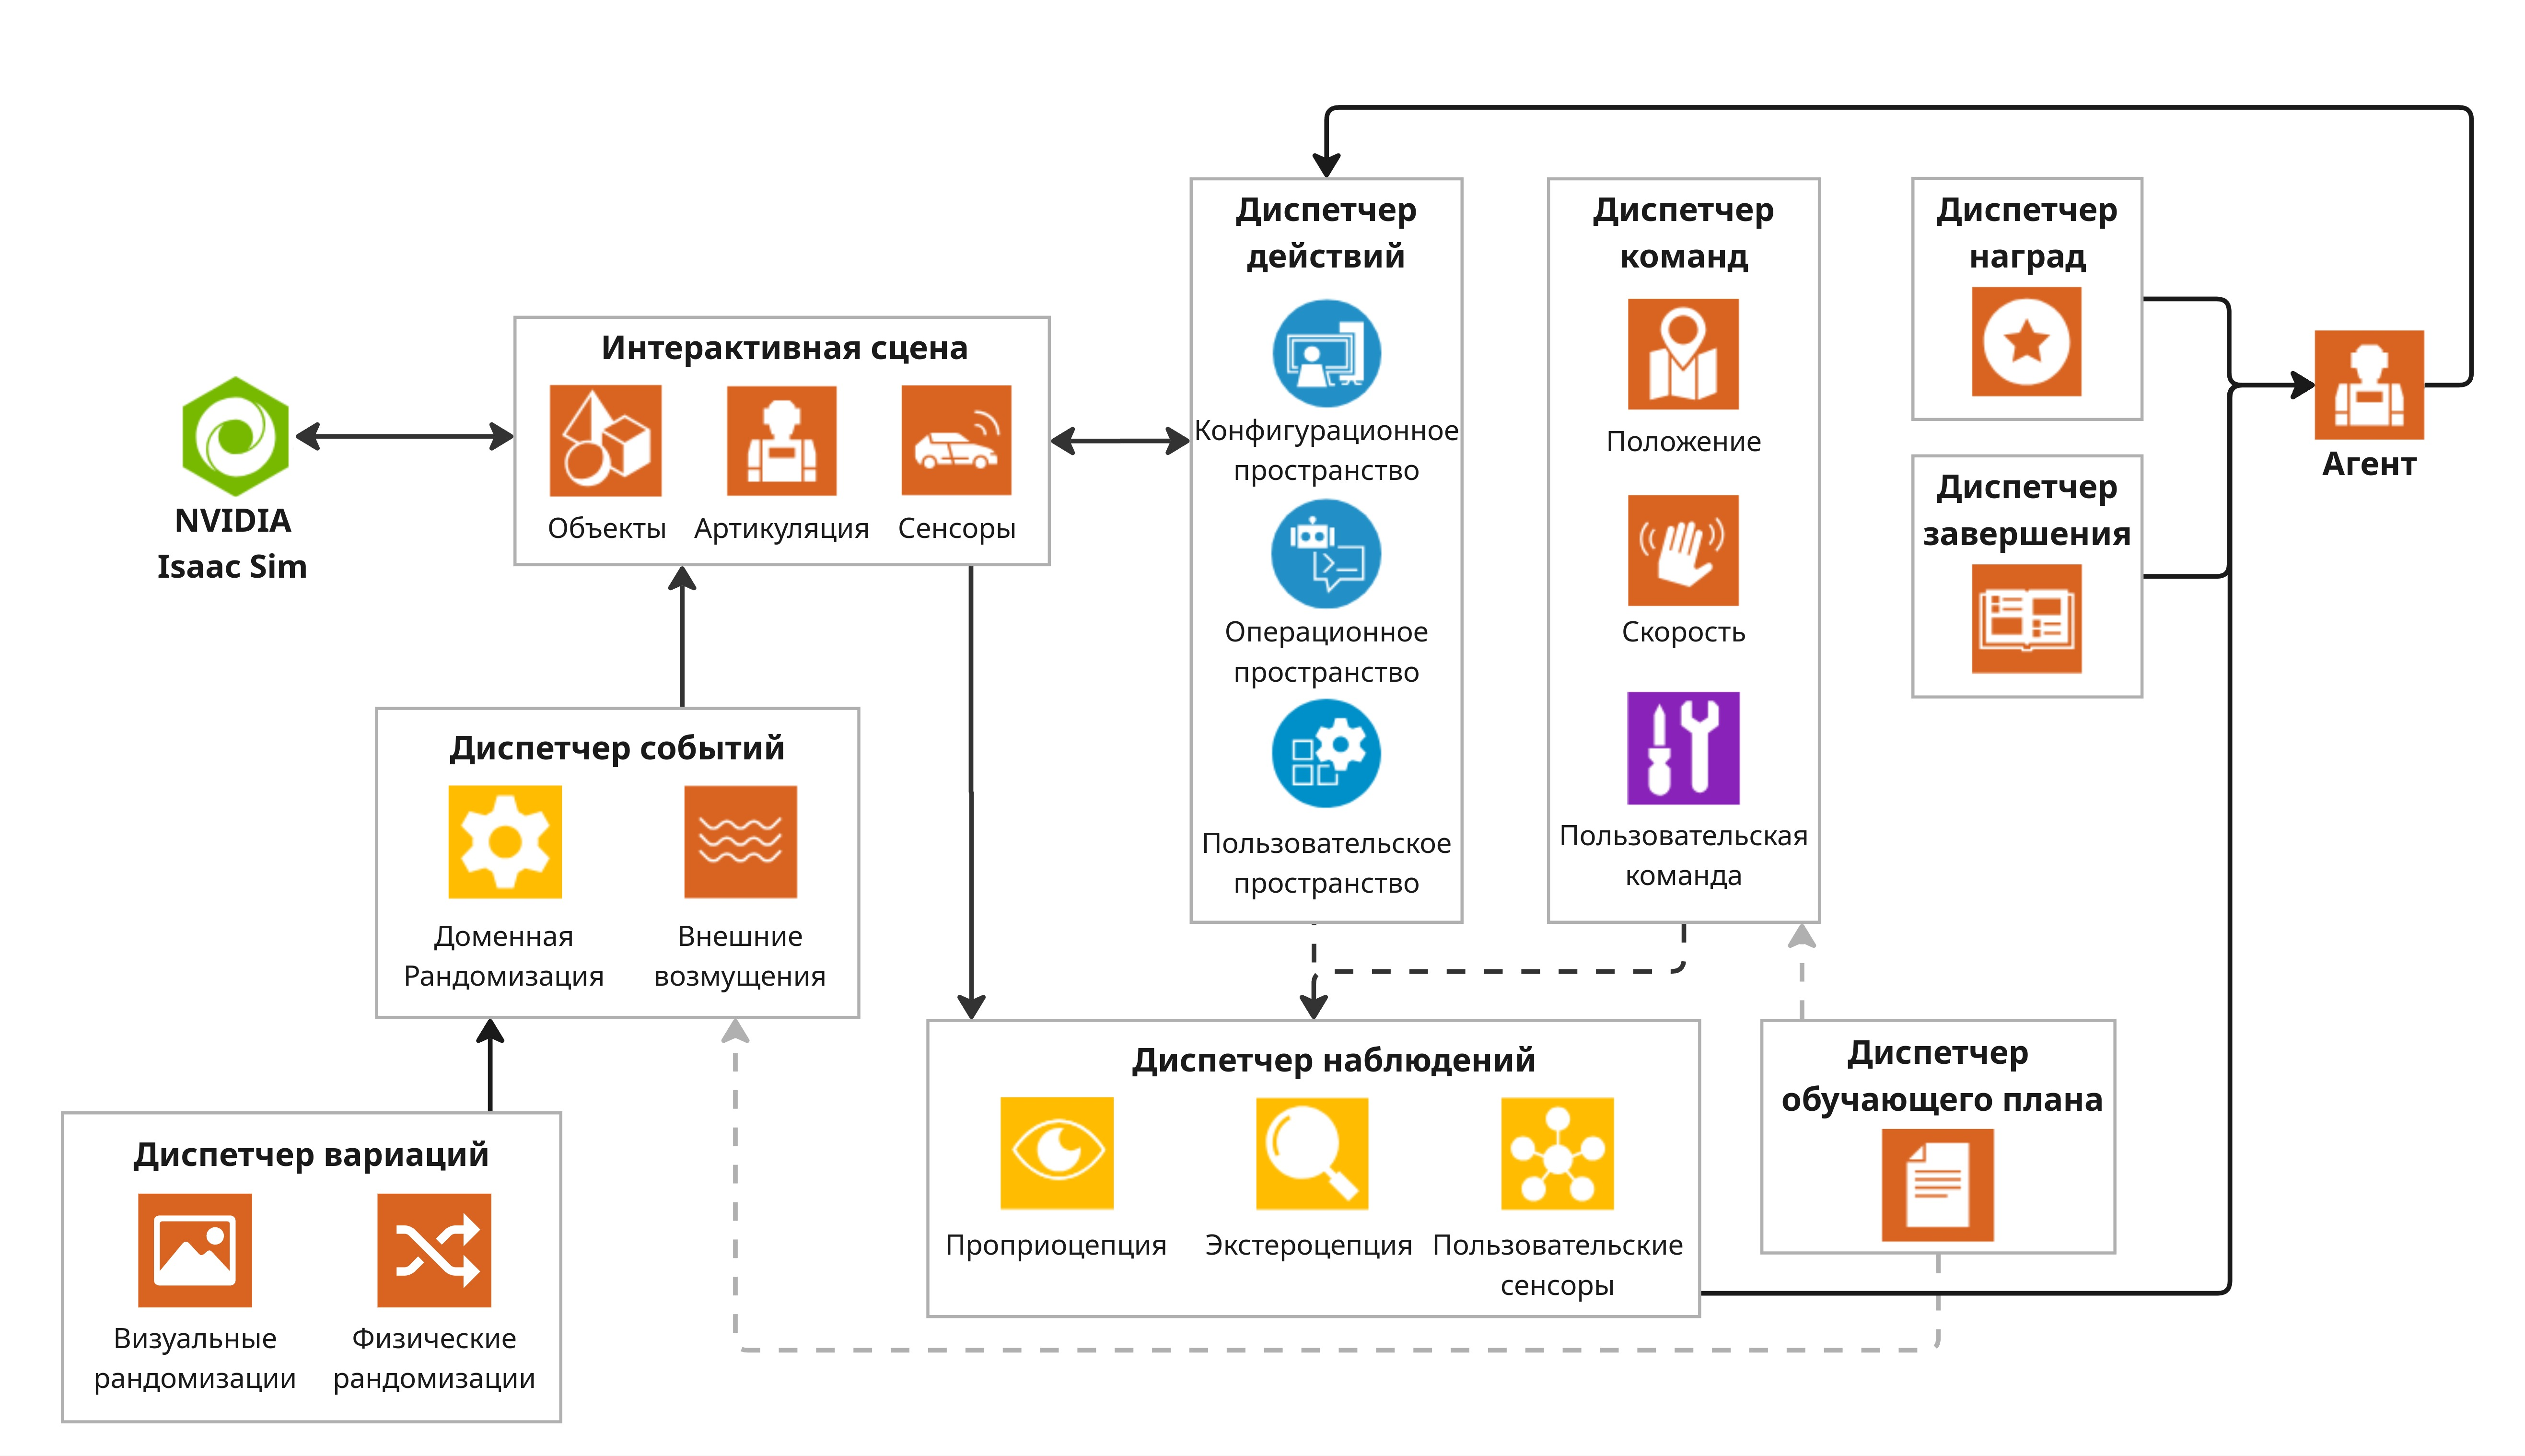
\includegraphics[width=1.0\textwidth]{images/Project Architecture.jpg}
            \caption{Архитектура метода}
            \label{fig:arch}
            \end{center}
        \end{figure}

        \subsection{Модуль варьирования параметров среды}
            Для каждой желаемой вариации создается экземпляр конфигурационного файла VariationCfg, который содержит всю необходимую информацию для применения соответствующей рандомизации, он содержит следующую информацию:

            \begin{itemize}
                \item Название вариации для отражения в отчетных материалах;
                \item Объект функции, которая непосредственно выполняет рандомизацию;
                \item Момент, когда должна применяться рандомизация (при запуске симулятора, в начале нового эпизода и т.д.);
                \item Дополнительные параметры, например, задающие распределение для рандомизированного параметра, распределение задается согласно пункту \ref{method_randomization}.
            \end{itemize} 

            Поля данного класса содержит всю необходимую информацию для создания экземпляров класса EventTerm, которые определяют события среды и регулируются диспетчером событий на верхнем уровне.  
            Чтобы хранить описания всех вариаций, а также настройки диспетчера вариаций, используется класс VariationManagerCfg который определяет конфигурацию для класса VariationManager, непосредственно управляющего всеми вариациями. Перед созданием среды, исходный конфигурационный файл диспетчера событий (EventCfg) передается диспетчеру вариаций, который добавляет экземпляры класса EventTerm, на основе экземпляров класса VariationCfg. Далее, модифицированный конфигурационный файл диспетчера событий передается конструктору среды.

            На нижнем уровне, ключевой является функция, применяющая рандомизацию. Если вариация подразумевает рандомизацию физических параметров, то обновленные параметры среды напрямую записываются в свойства соответствующих объектов и учитываются уже вначале следующего эпизода. Вариация визуальных составляющих является более сложным процессом, ввиду особенностей работы симулятора Isaac Sim. Для реализации подобного функционала в симуляторе представлен фреймворк Omniverse Replicator, предназначенный для разработки пользовательских процессов генерации синтетических данных. Данный фреймворк активно используется при реализации доменной рандомизации в Isaac Sim и поэтому является наиболее уместным для модуля варьирования параметров среды. 
            
        \subsection{Настройка выхода модели}

            Фреймворк IsaacLab поддерживает библиотеки обучения с подкреплением RL-Games \cite{rl-games2021}, RSL-RL \cite{rudin2022learning}, SKRL \cite{serrano2023skrl}, Stable-Baselines3 \cite{stable-baselines3} и библиотеку имитационного обучения Robomimic \cite{robomimic2021}. Модели обученные с помощью этих библиотек могут быть напрямую интегрированы в разработанный программный модуль. Однако, рекомендуемый способ настройки выхода модели независимо от используемой библиотеки является развертывание модели в отдельном виртуальном контейнере, с помощью программного обеспечения Docker \cite{merkel2014docker}. В таком случае, исключаются проблемы с синхронизацией версий зависимых пакетов для разработанного модуля и для исследуемой модели, что позволяет исследовать большой кластер моделей, не нарушая работу модуля. Коммуникация между моделью и модулем оценивания робастности осуществляется при помощи библиотеки FastAPI \cite{Ramirez_FastAPI}. Данные передаются по локальной сети через стандартный протокол HTTP.

        \subsection{Реализация алгоритма оценивания робастности модели}

            Алгоритм оценивания робастности, на основе определенных в \newline VariationManagerCfg вариациях, последовательно применяет их к среде, модифицируя конфигурационный файл диспетчера событий. В начале каждого эпизода применяются рандомизации согласно заданным параметрам, таким образом каждый эпизод генерируется новая вариация исходной среды. Некоторые параметры среды определяются при запуске симулятора и не могут быть изменены в процессе, не нарушив стабильность работы программного обеспечения. В таком случае, для генерации новой вариации среды приложение симулятора автоматически перезапускается. Исследуемая модель запускается в среде $N$ раз и подсчитываются метрики эффективности, определенные пунктом \ref{method_robust}. Метрики сохраняются в файл, с указанием индекса вариации и измеренным показателем эффективности. Полученные для каждой вариации метрики обрабатываются, и подсчитывается итоговая оценка робастности, согласно описанию в пункте \ref{method_robust}.
        
            Ссылка на программную реализацию представлена в \hyperref[sec:program]{приложении В}.
